\section{Incremental Clustering}
\label{sect:incremental-clustering}

The incremental clustering phase translates changes of the input graph to changes of its cluster graph: it takes a sequence of operations that was applied to a previous version of the input graph and its cluster graph as input and outputs a (potentially empty) sequence of operations to be applied to the cluster graph:

\begin{figure}[H]
	\centering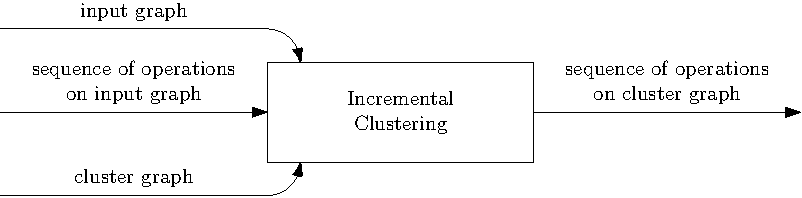
\includegraphics[width=0.8\textwidth]{Resources/DynamicPipeline-IncrementalClustering.pdf}
	\caption{Input and output of the incremental clustering phase.}
	\label{fig:dynamic-pipeline-incremental-transformation}
\end{figure}

The cluster graph of the previous version of the input graph is needed because the output sequence is tailored to a specific cluster graph. It has to be specified as input rather than being part of the output because we want to continue propagating the changes through the pipeline and apply it to a product of a non-incremental phase eventually. If we didn't specify these products as input to the incremental phases, the sequence of operations might not be compatible with the products of the non-incremental phases.

We assume that in concrete implementations, the cluster graph preserves enough information about the input graph to allow for incremental clustering. For example, the cluster graph might keep track of which vertices of input graph its clusters contain. \todo{Or do we want to formalize that with explicit mathematical definitions of cluster graph etc.?}

The following operations on the cluster graph can be output and are sufficient to turn any cluster graph into a different one:
%
\begin{itemize}
	\setlength\itemsep{-0.5em}
	\item change a vertex' weight
	\item change an edge's weight
	\item add a vertex with arbitrary weight and edge weights to existing vertices
	\item remove a vertex
\end{itemize}
%
Note that because the cluster graph is a complete graph, we are not allowed to add or remove individual edges and adding a new vertex to the cluster graph implicitly adds edges to all existing vertices.
